\documentclass{article}
\title{Controller Design and Simulation for Mobile Inverted Pendulum (mIp)}
\author{Yuhao Lian}
\usepackage{indentfirst}
\usepackage{amsmath}
\usepackage{amssymb}
\usepackage{graphicx}
\graphicspath{{D:/GitHub/MAE280A-Linear-System-Theory/Figures/}}
\begin{document}
\maketitle
\section{Introduction}
This work is based on Zhu Zhuo's Master Thesis on controller designing for a Mobile Inverted Pendulum (mIp). We will first examine his controller's performance by running various tests in Simulink. Then we will try to design a controller using state-estimate feedback with parameter experimentally determined by Zhu Zhuo. Lastly we will conduct various tests on our controller and further discuss its performance.
\section{System Modeling and Linearization}
In Zhu's Master Thesis, he first introduced mIp robots and classic control methods for the robot. Then he modeled the system with parameters \textit{a,b,c,d,e} and \textit{j}. The robot body's angle of rotation is defined as $\theta$ and the angle of the wheels is defined as $\phi$. Voltage input is $V(t)$.Two equilibrium points were identified as the following:
\begin{center}
Equilibrium 1: $\theta(t)$=0, $\dot{\theta}(t)$=0, $\dot{\phi}(t)$=0,\textit{V(t)}=0\\
Equilibrium 2: $\theta(t)$=$\pi$, $\dot{\theta}(t)$=0, $\dot{\phi}(t)$=0,\textit{V(t)}=0
\end{center}
The second equilibrium point is at stable where the robot body is hanging straight down. The first equilibrium is unstable with robot body pointing up. We are interested in stabilizing the first equilibrium using our controller. The state space realization of the system is shown below:
$$
\begin{pmatrix}
x_1\\
x_2\\
x_3 
\end{pmatrix}
=
\begin{pmatrix}
\dot{\theta}(t)\\
\dot{\phi}(t)\\
\theta(t)
\end{pmatrix}
,\
\begin{pmatrix}
y_1(t)\\
y_2(t)
\end{pmatrix}
=
\begin{pmatrix}
\dot{\theta}(t)\\
\dot{\phi}(t)
\end{pmatrix}
,\
u(t)=V(t)
$$
The system here is nonlinear. Linearization around Equilibrium 1 is performed. The linearized system looks like this:
\begin{equation}
\dot{
\begin{pmatrix}
x_1(t)\\[6pt]
x_2(t)\\[6pt]
x_3(t)
\end{pmatrix}
}
=
\begin{pmatrix}
-\frac{(a+b)j}{-b^2+ac} & \frac{(a+b)j}{-b^2+ac} & \frac{ad}{-b^2+ac}\\[6pt]
-\frac{(b+c)j}{b^2-ac} & \frac{(b+c)j}{b^2-ac} & \frac{bd}{b^2-ac}\\[6pt]
1 & 0 & 0\\
\end{pmatrix}
+
\begin{pmatrix}
-\frac{(a+b)e}{-b^2+ac}\\[6pt]
\frac{(b+c)e}{-b^2+ac}
\end{pmatrix}
\cdot
u(t)
\end{equation}
After conducting experiments of the mIp to get more accurate values of the parameters, Zhou came up with the following values for matrix $\boldsymbol{A,B,C,D}$ in the state space model:
\begin{equation}
\begin{gathered}
A=
\begin{pmatrix}
-13.692 & 13.692 & 128.381\\
21.023 & -21.023 & -83.514\\
1 & 0 & 0
\end{pmatrix}
,\
B=
\begin{pmatrix}
-74.101\\
113.775\\
0
\end{pmatrix}
\\
\\
C=
\begin{pmatrix}
1 & 0 & 0 \\
0 & 1 & 0
\end{pmatrix}
,\
D=
\begin{pmatrix}
0\\
0
\end{pmatrix}
\end{gathered}
\end{equation}
\section{State Estimate Feedback Controller}
\paragraph{Equilibrium Test}
Our main focus is to design a state estimate feedback controller for the system. Here we use pole placement method to stabilize the system. Eigenvalues of matrix $A$ is $-34.0470$, $7.7498$ and $-5.4178$. We can see that one eigenvalue is in the right half plane, which makes the system unstable. The goal of our controller is to place all of A's eigenvalue on the left half plane. This could be done by adding a state feedback controller by pole placement. Since not all states could be measured directly, an observer is needed to estimate the states in order to provide the best feedback. This is done by choosing the $K$ and $L$ matrix that places poles at a desired value. This is done with MATLAB command $K$=place($A$,$B$, $Poles_1$) and $L$=place($A'$,$C'$, $Poles_2$)' where $A'$ and $C'$ denotes transpose of matrix $A$ and $C$, respectively. $Poles_1$ and $Poles_2$ denotes where we would like the poles to be placed. The Simulink model was created to simulate the performance of the controller. The controller will be discrete time therefore discretization has to be performed after we construct the controller.After a few trials and errors, $Poles_1$ were selected to be ${-30,-7,-4.5}$ which are about 90\% of the eigenvalues of $A$. $Poles_2$ were chosen to be ${-150,-35,-22.5}$ which are 10 times faster than $Poles_1$. We examine the performance of our controllers by running it in Simulink shown below in Figure 1. 
\begin{figure}[h!]
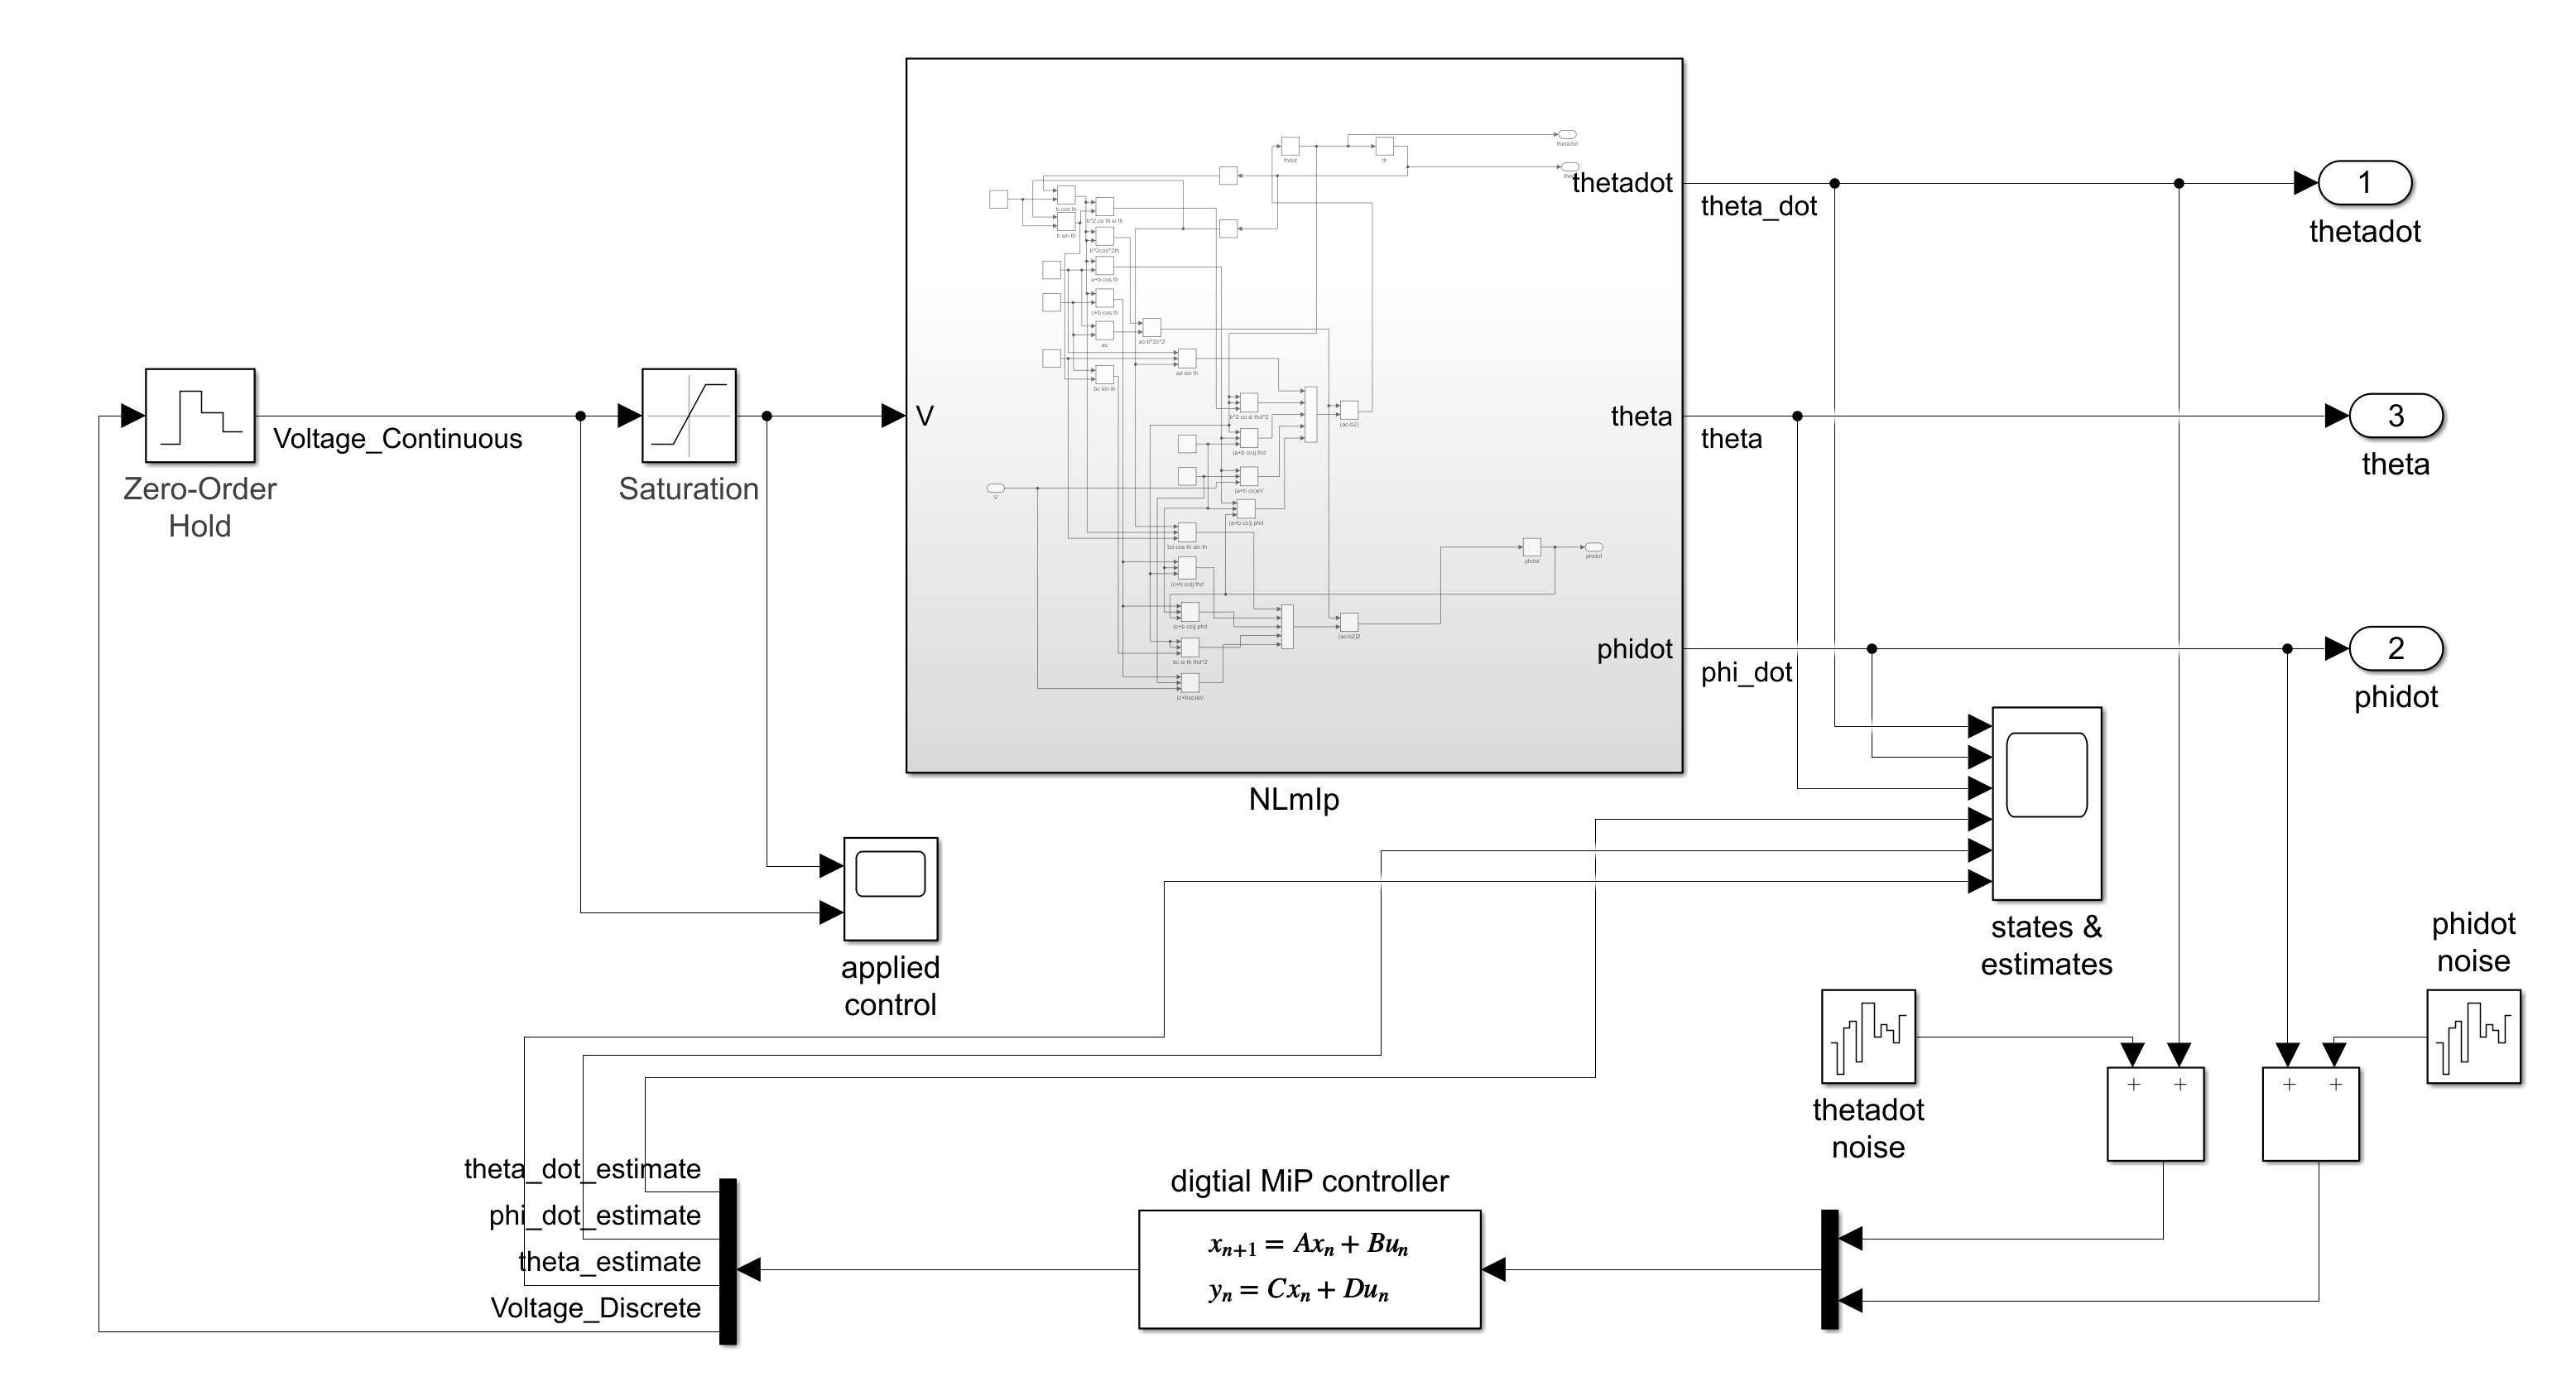
\includegraphics[width=0.8\textwidth]{Simulink_Model}
\centering
\caption{Simulink Model of the mIp robot.The NLmIp block represents the state equations (1)}
\centering
\end{figure} 
We can see that there are two blocks that simulate the noise added on to $\dot{\theta}(t)$ and $\dot{\phi}(t)$. First we turn off the noise by setting both noise power to 0. The initial states can be changed within the NLmIp block. The initial states are all set to 0 for equilibrium test. The test result is shown below in Figure 2 and Figure 3. We expect all the states and estimated state to stay at 0 as well as the voltage output from our controller.
\begin{figure}[h!]
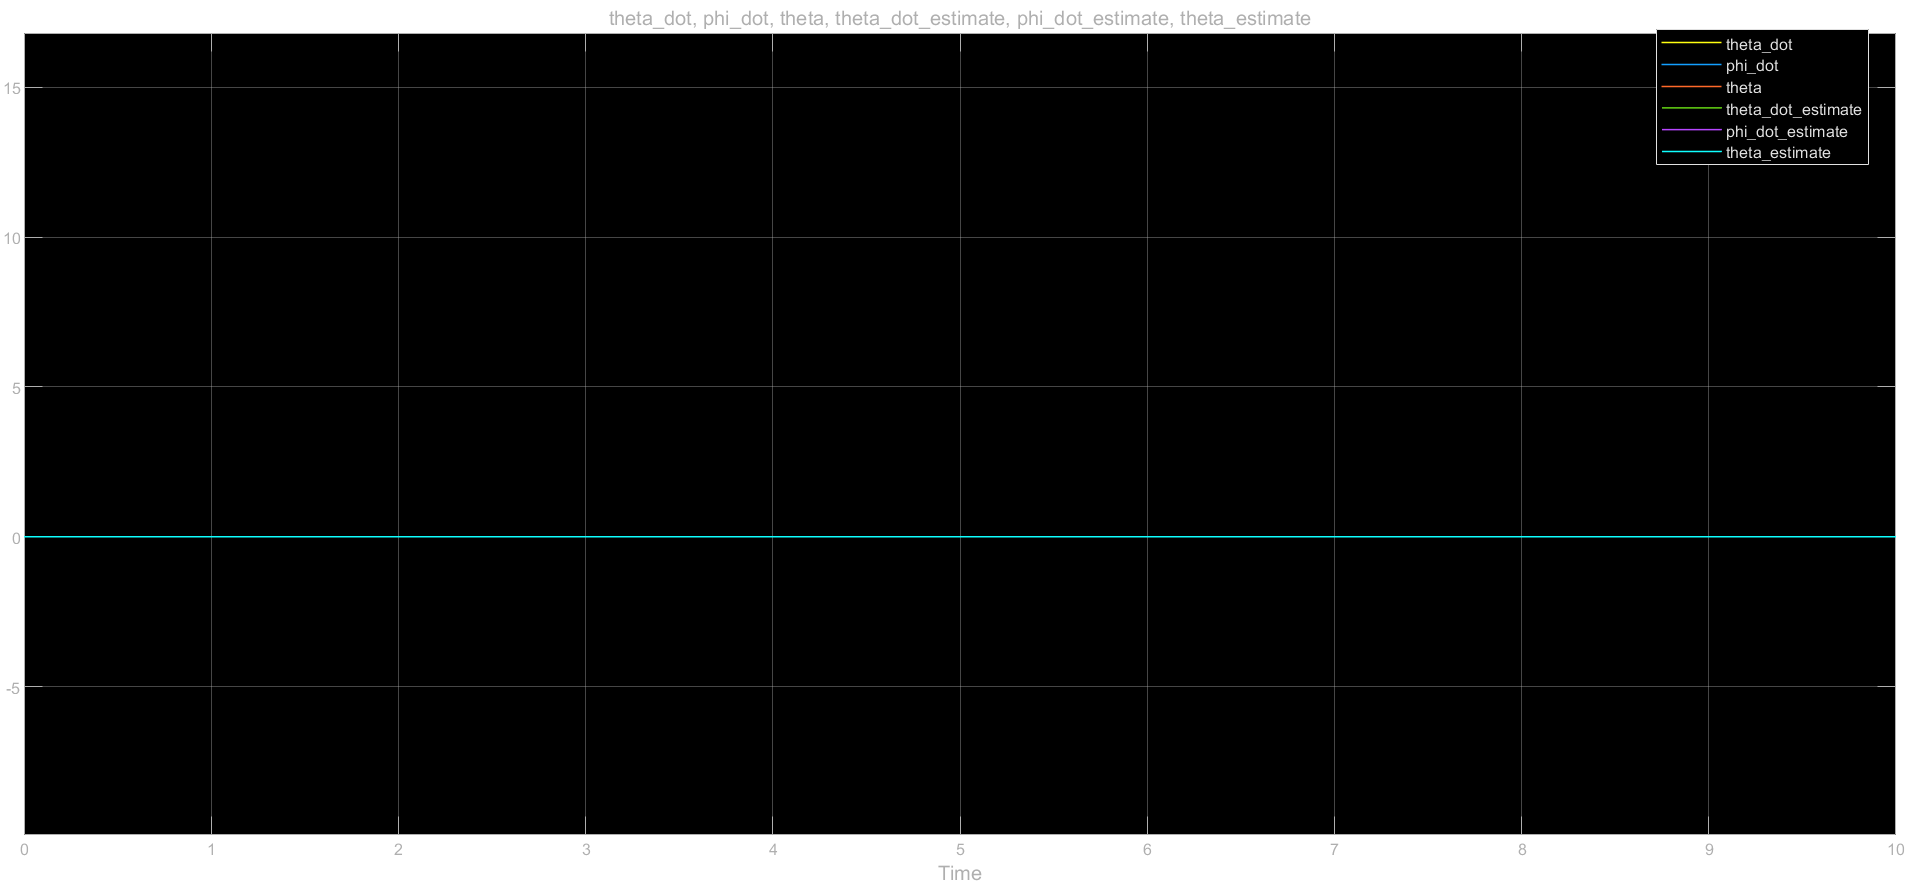
\includegraphics[width=0.8\textwidth]{Equilibrium_Test_States}
\centering
\caption{The plot above shows states $\dot{\theta}$, $\dot{\phi}$ and $\theta$ and their estimates.}
\end{figure}
\begin{figure}[h!]
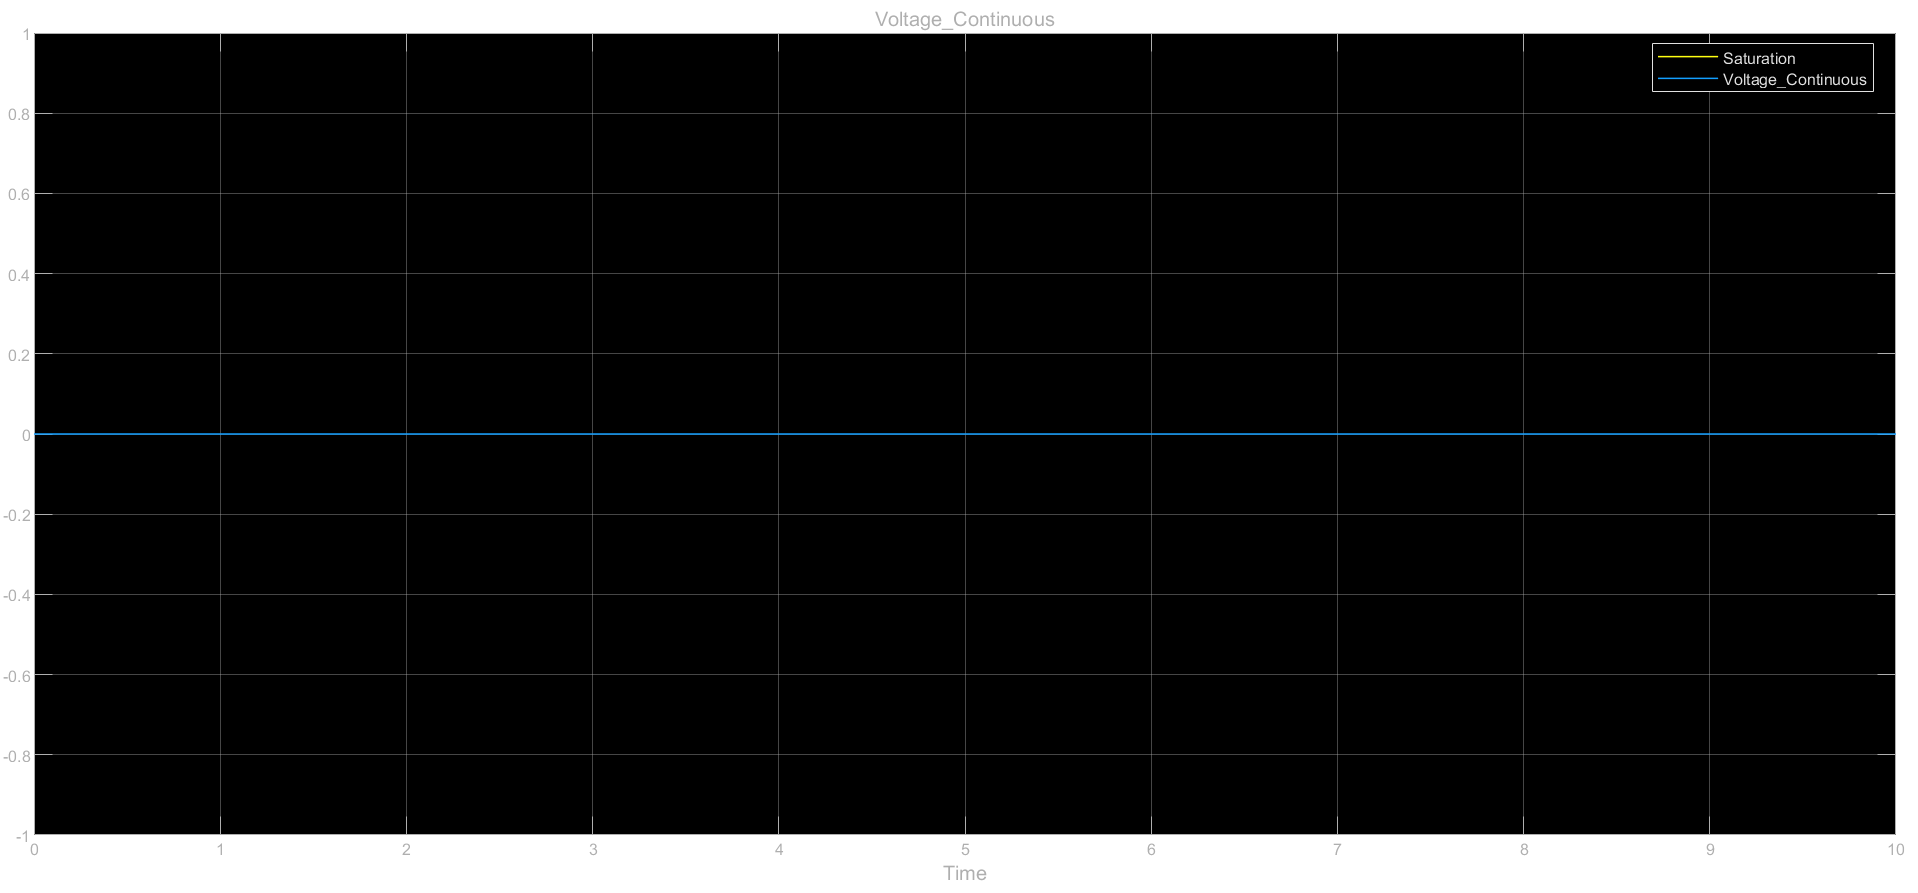
\includegraphics[width=0.8\textwidth]{Equilibrium_Test_Voltage}
\centering
\caption{The plot below shows the Voltage output $u$ from our controller.}	
\end{figure}
\paragraph{Stabilization Test}
Now we need to test our controller's ability to stabilize the system when the initial condition is non-zero. Also we want to find out the limit of our controller. First the initial condition of $\theta_0=0.1\ rad$ with all the noises turned off. The results are shown in Figure 4 and 5 with zoomed-in time span from 0 to 2 seconds. First we look at the plot of states, our state estimator quickly converged to the actual states which ensures the state feedback are based on states with minimized error. Then we can see that all states and estimated states converge to 0 quickly, within less than 1.5 seconds. We also have to check the voltage output from our controller to make sure it is in the limit of $[-6V,6V]$. From the results shown in both plots we can conclude that our controller works well with the initial condition $\theta_0=0.1\ rad$.\par
\begin{figure}[h!]
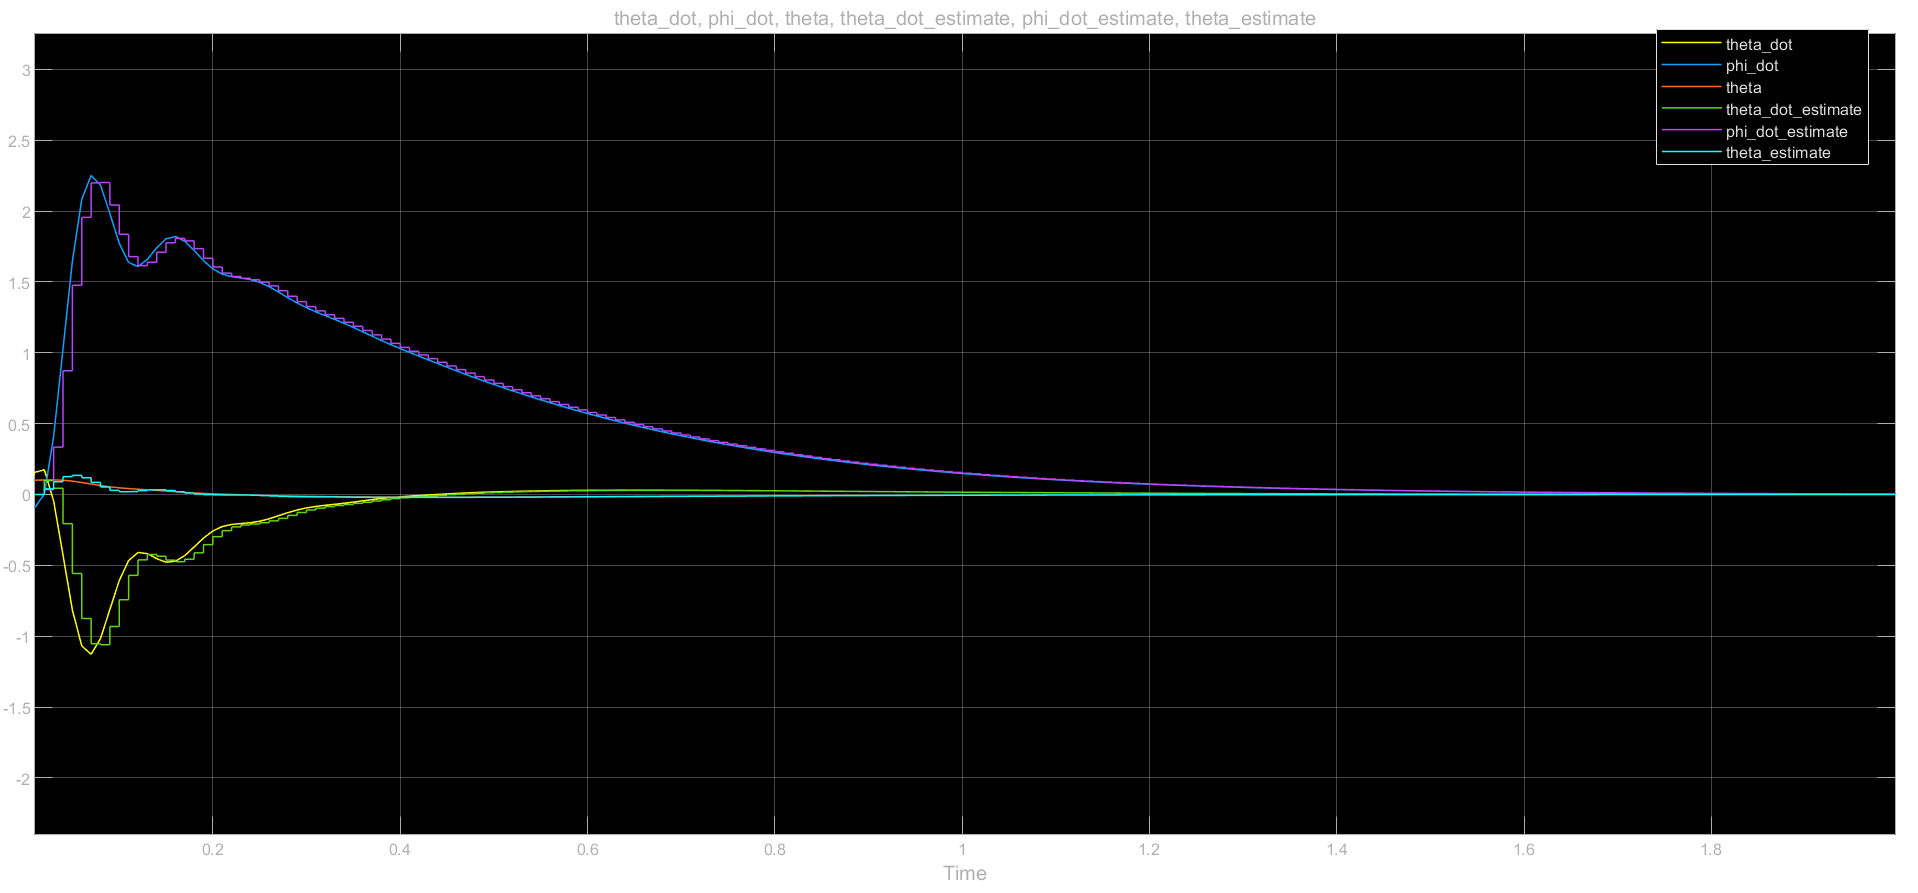
\includegraphics[width=0.8\textwidth]{Test_States}
\centering
\caption{Actual and estimated state response to $\theta_0=0.1\ rad$}
\end{figure}
\begin{figure}[h!]
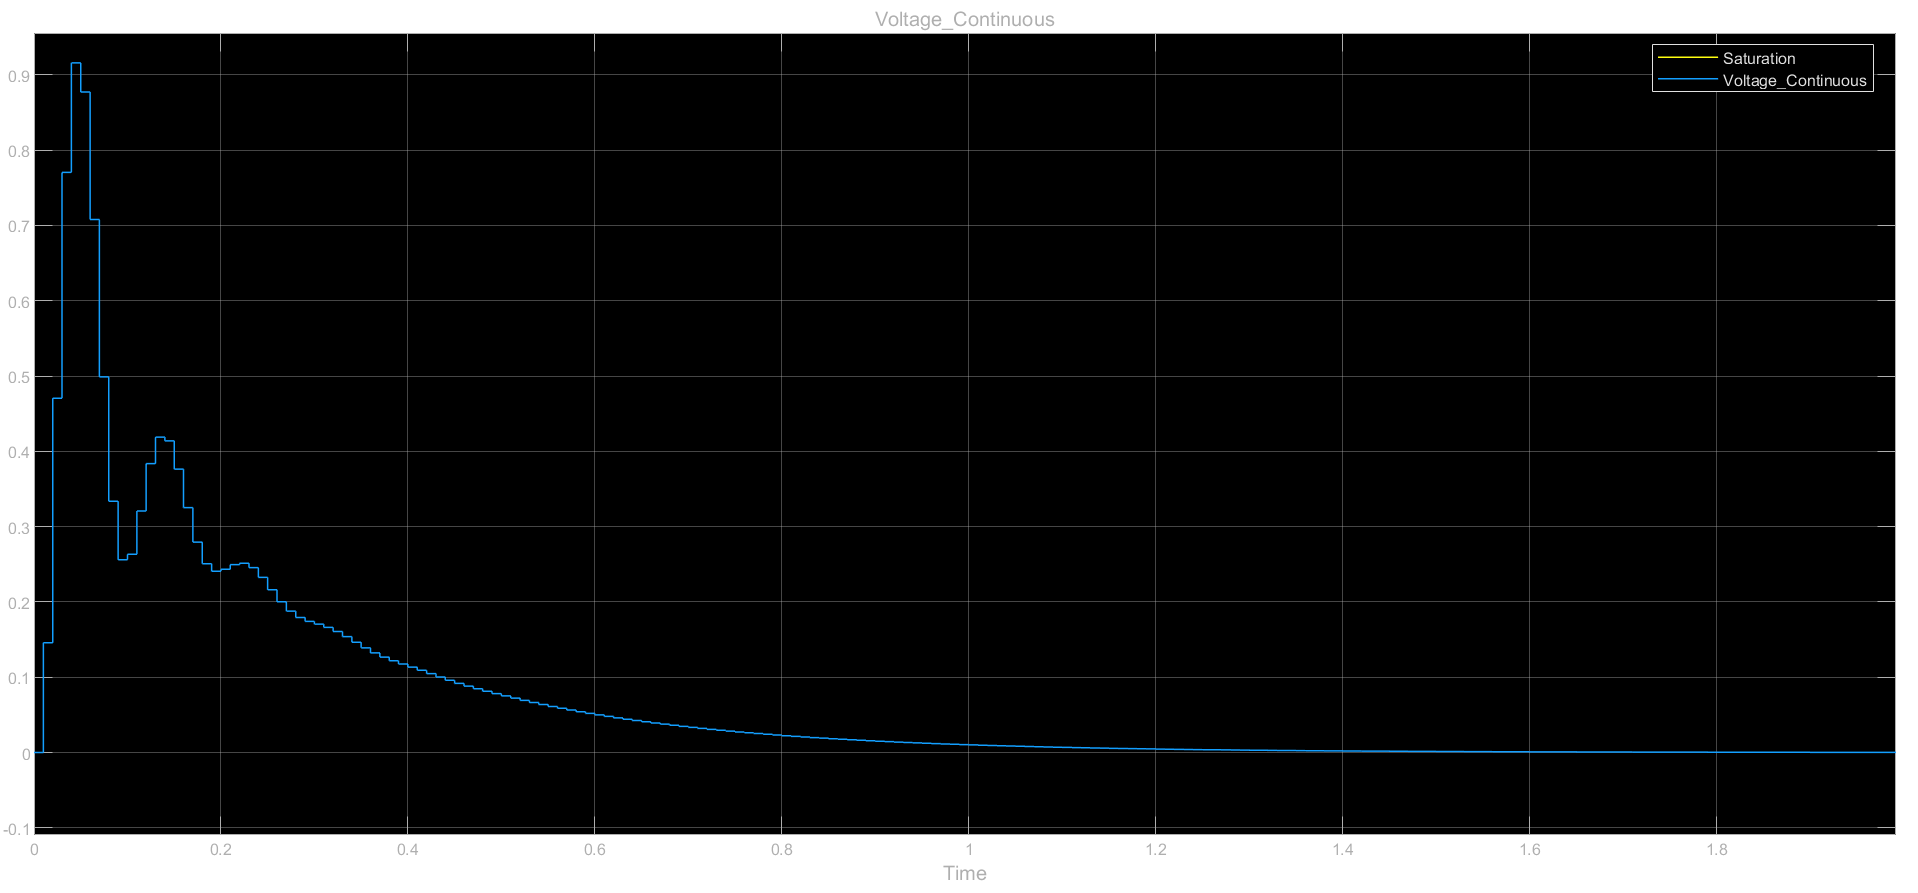
\includegraphics[width=0.8\textwidth]{Test_Voltage}
\centering
\caption{Voltage output of controller}
\end{figure}
With a few trials on the initial condition, we found out the limit of our controller. The maximum value of $\theta_0$ that the controller can stabilize is 0.57 $rad$. However, under this initial condition, the maximum voltage exceeds 6V and the system is saturated. We then tuned down $\theta_0$ to make sure the voltage output is within the range of $[-6V,6V]$. The maximum $\theta_0$ that our controller can handle without saturation is 0.52 $rad$. The state responses and controller output are shown in Figure 6 and Figure 7. Both plots are zoomed in to focus on the first 2 seconds of the system response.\par   
\begin{figure}[h!]
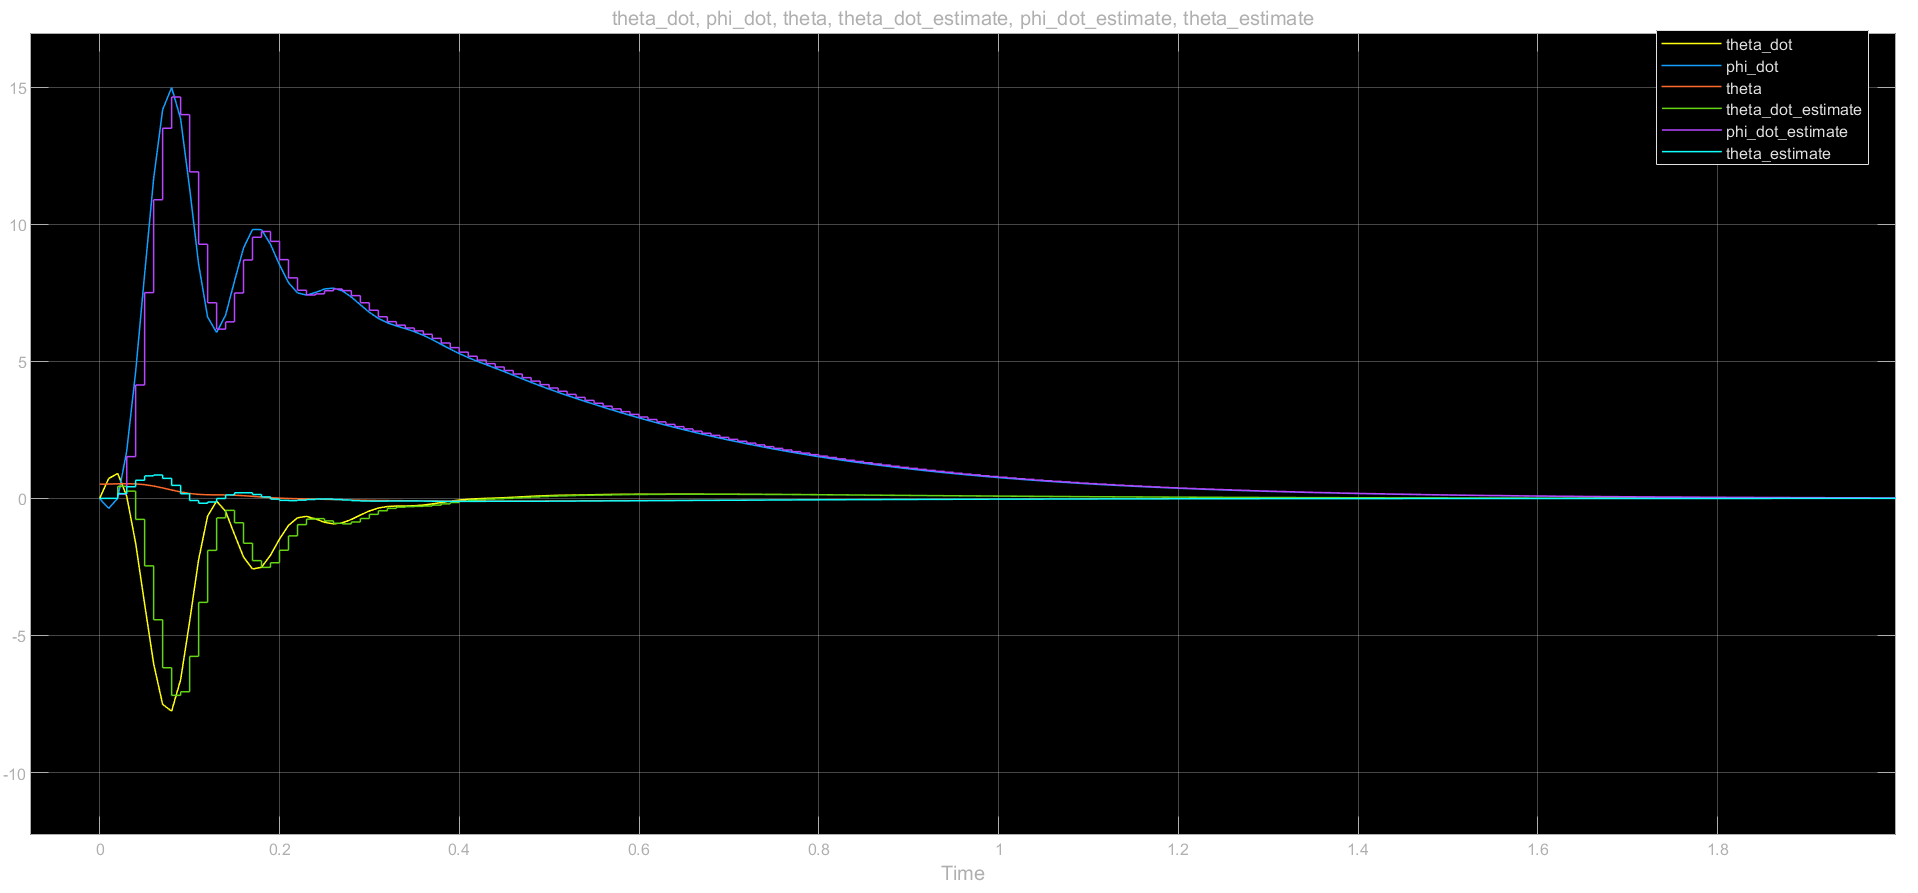
\includegraphics[width=0.8\textwidth]{Max_States}
\centering
\caption{Actual and estimated state response to $\theta_0=0.52\ rad$}
\end{figure}
\begin{figure}[h!]
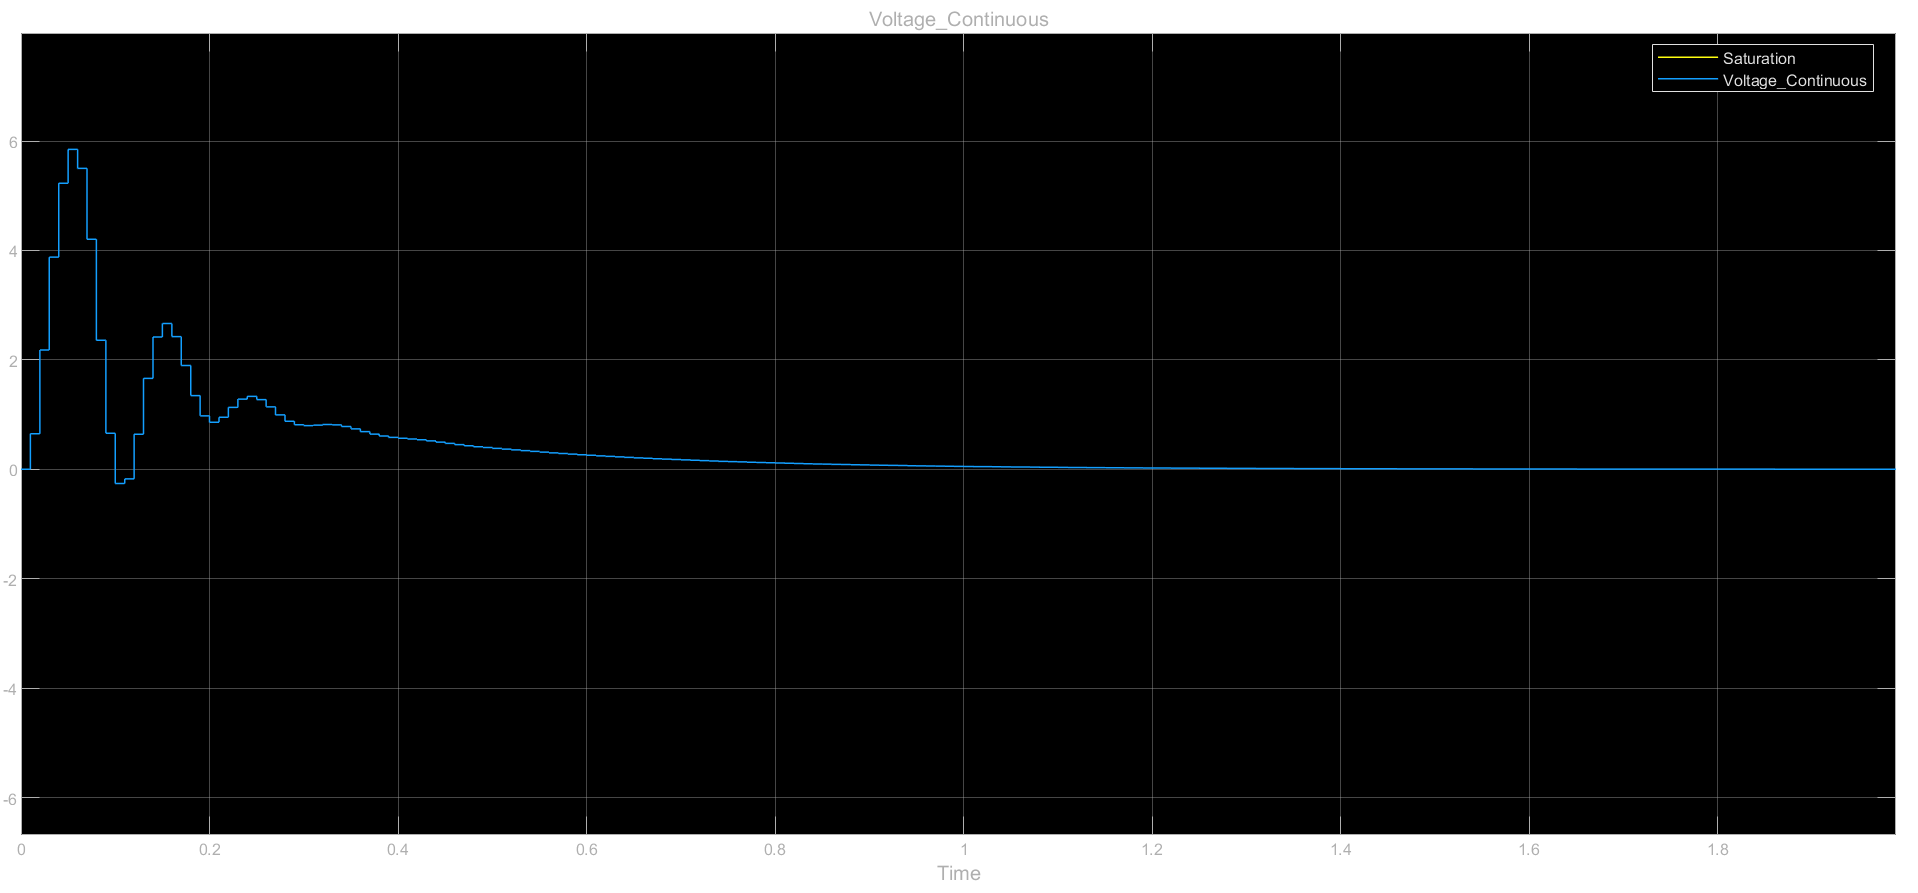
\includegraphics[width=0.8\textwidth]{Max_Voltage}
\centering
\caption{Voltage output from the controller}
\end{figure}
With the performance and limitation of our controller determined, we now turn on the noise power to see how our controller handles noisy inputs. With noise power of $\dot{\theta}$ and $\dot{\phi}$ both set to 0.0001, we have the results below shown in Figure 8 and 9. Both plots have time span from 0 to 10 seconds from now because we want to check the noise effects within the full time span. We can see from the plot that our controller still successfully stabilized the system within the saturation limits. 
\begin{figure}[h!]
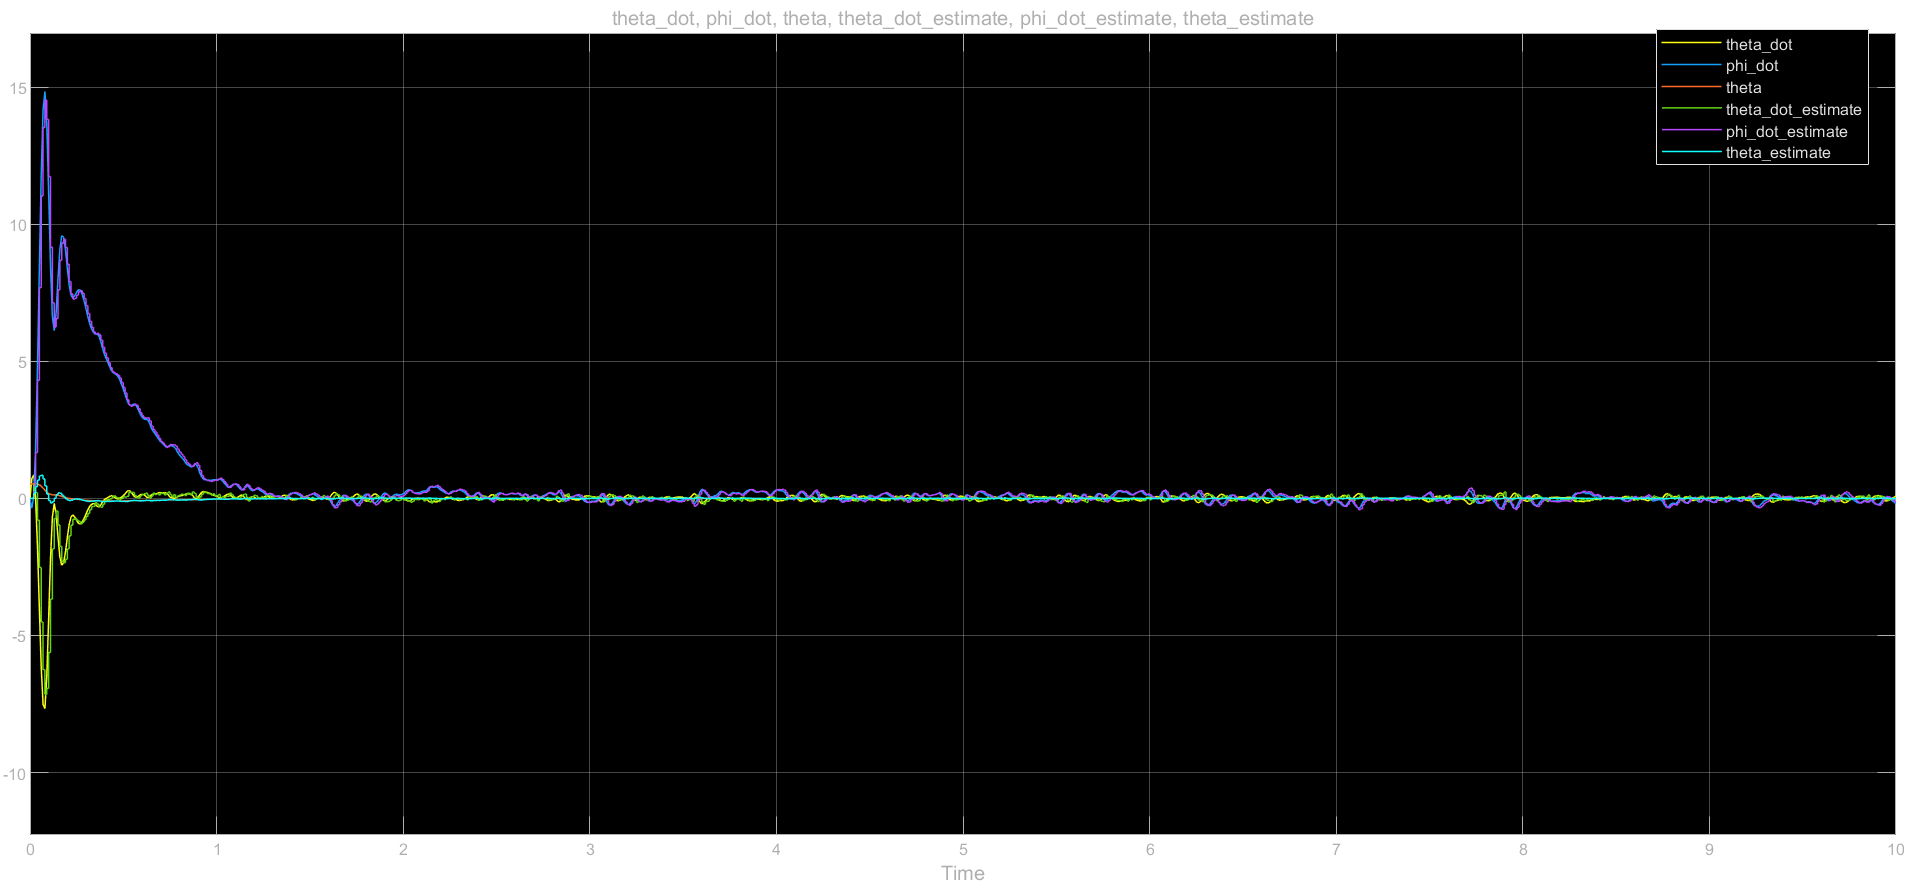
\includegraphics[width=0.8\textwidth]{Noisy_Max_States}
\centering
\caption{Actual and estimated state response to $\theta_0=0.52\ rad$ with noise turned on}
\end{figure}
\begin{figure}[h!]
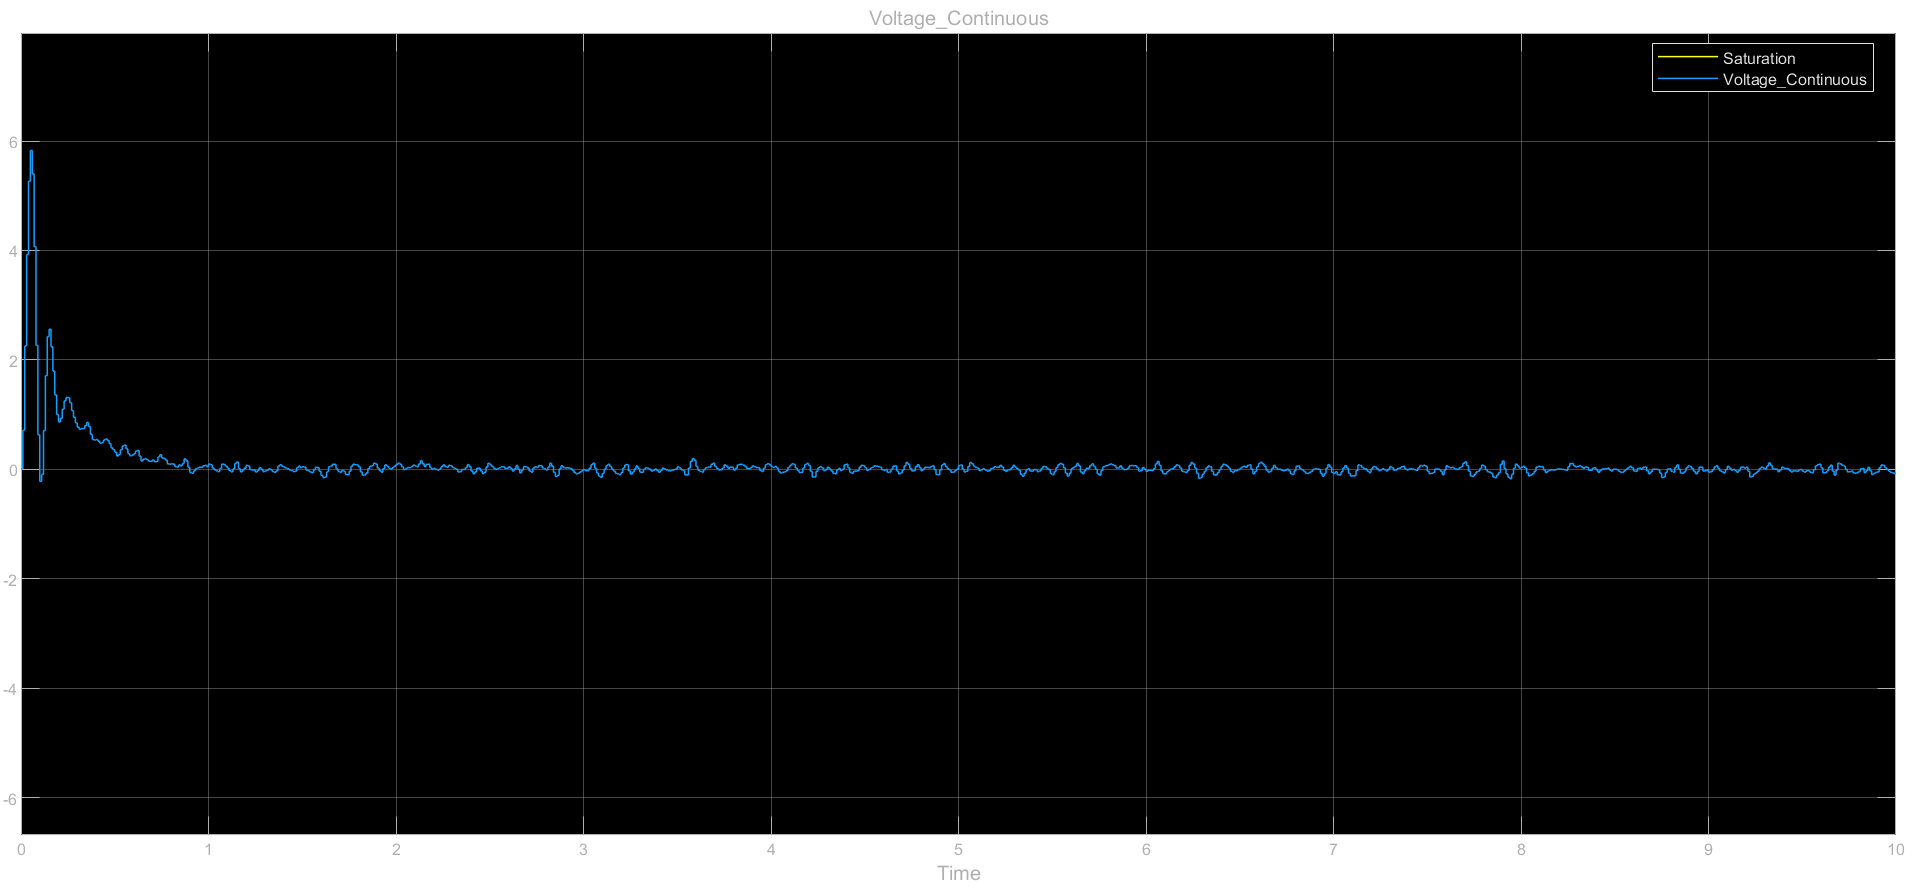
\includegraphics[width=0.8\textwidth]{Noisy_Max_Voltage}
\centering
\caption{Voltage output from the controller with noise turned on}
\end{figure}

\end{document}